\documentclass{article} 
\usepackage{tikz} 
\usepackage{graphicx}
\usepackage{caption}
\begin{document} 

\textbf{Exercitiul 3. (a1) }

La fiecare pas al algoritmului, functia $Search()$ alege arcul $e = ij$ cu costul minim $u_i + a_{ij}$, unde $i \in S,j \notin S$. Daca adaugam un nod la $S$, cu siguranta stim si costul lui minim $u_i$. Cum algoritmul alege doar nodul cu costul \textbf{minim} la fiecare iteratie (\textbf{while}), nodurile sunt adaugate la $S$ crescator in functie de cost.

\begin{figure}[h!]
  \centering
  \renewcommand{\thefigure}{}
  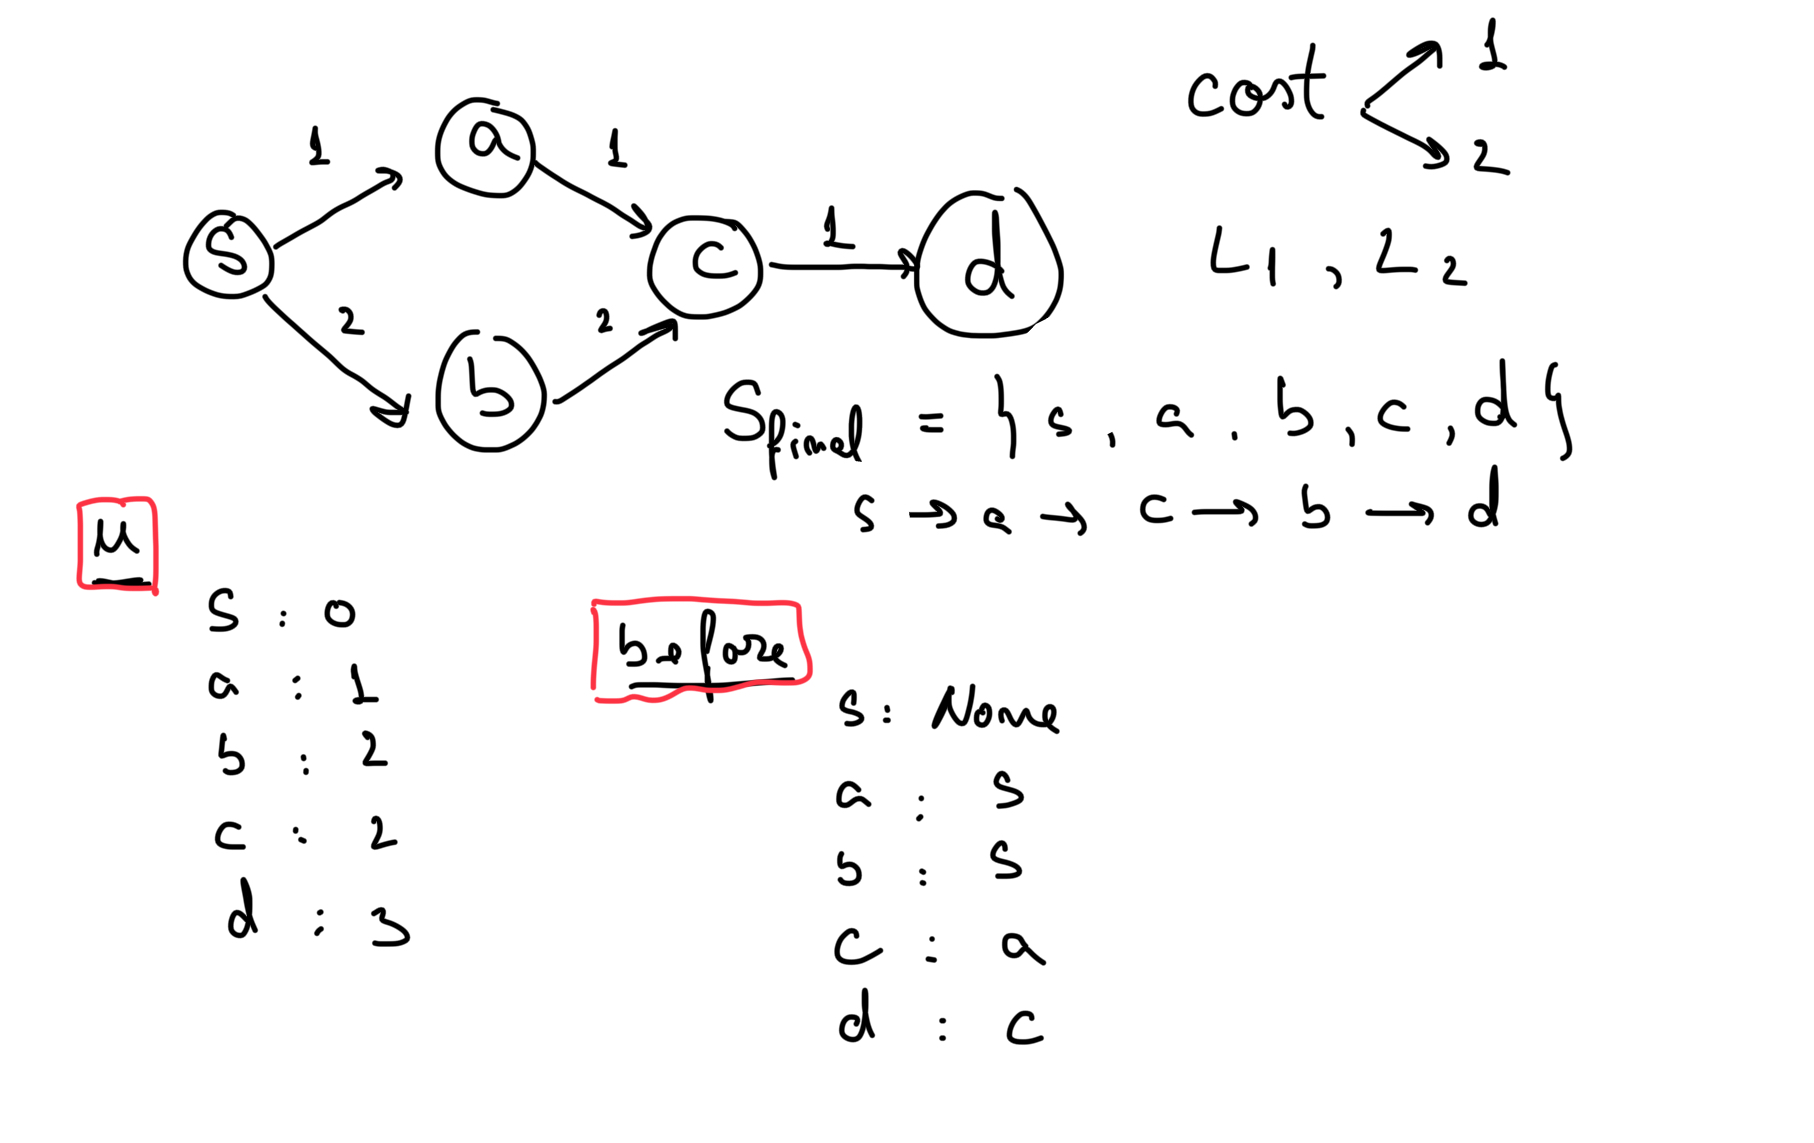
\includegraphics[width=0.7\textwidth]{example_digraf.jpg}
  \caption{Costurile minime si predecesorii obtinuti dupa executia algoritmului.}
  \label{fig:my_image}
\end{figure}

In exemplul de mai sus, ordinea in care adaugam la S este urmatoarea : $[a]$, $[a, c]$, $[a, c, b]$, ... $Search()$ cauta nodul minim dintre $(s, b)$ si $(a, c)$ si alege $(a, c)$ pentru ca are costul minim. Astfel $c$ va fi adaugat la $S$ inaintea lui $b$.

Asadar, nodurile sunt adaugate la $S$ in ordine crescatoare a costurilor minime.

\textbf{Exercitiul 3. (a2) }

Presupunem ca exista doua arce $(i,j)$ si $(i',j')$ in $L_h$ pentru care costul minim pana la nodul $i$ este mai mic decat costul minim pana la nodul $i'$, adica $u_i < u_{i'}$, dar in $L_h$ arcul $(i',j')$ apare inaintea lui $(i,j)$.

Algoritmul $Dijkstra$ adauga nodurile in $S$ in ordine crescatoare a costurilor $u$. Asta inseamna ca un nod $i$ pt. care $u_i < u_{i'}$ va fi adaugat in $S$ inaintea lui $i'$

Daca $u_i < u_{i'}$, atunci $(i,j)$ va fi adaugat inaintea lui $(i',j')$ pt ca in $S$ adaugam $i$.

Conform presupunerii, $(i',j')$ apare inaintea lui $(i,j)$, ceea ce inseamna ca $i'$ a fost procesat inainte lui $i$. \textbf{IMPOSIBIL}, pentru ca stim ca $u_i < u_{i'}$ si ca nodurile sunt adaugate in $S$ in ordinea costurilor minime. 

Contradictie, nu putem avea $u_i < u_{i'}$ si $i'j'$ inaintea lui $ij$ in coada.
Presupunearea facuta este falsa, asadar arcele din coada $L_h$ sunt ordonate cum trebuie, in ordine crescatoare a costurilor minime $u$.

\textbf{Exercitiul 3. (a3) }

Algoritmul adauga arcele in cozi : $if (a_{si} = y_h)$ then $L_h.push(si)$

La fiecare iteratie din bucla $while$ : un nod $j^*$ este ales si adaugat la $S$, toate arcele $(j^*,j)$ catre noduri $j \notin S$ si care au cost $y_h$ sunt adaugate in $L_h$.

Cum se mentine structura la fiecare iteratie : un nod $j^*$ este in inclus in $S$, ne asiguram ca toate arcele incidente $(j^*,j)$, $j \notin S$ si $a_{j*j} = y_h$ sunt adaugate in $L_h$. In fiecare moment, daca avem $(i,j)$ cu $i \in S$, $j \notin S$ si $a_{i*j} = y_h$, atunci $(i,j)$ prezent in $L_h$.

Asadar, se verifica proprietatea ceruta.

\textbf{Exercitiul 3. (a4) }

Pentru a verifica proprietatea voi folosi o demonstratie prin inductie asupra iteratiilor algoritmului.

\textbf{Cazul de baza, P(0)} : $S=[s]$ (avem doar nodul de start), iar $u_S=0$

$\forall j$ adiancent cu $s$, $u_j$ = $a_{sj}$ (care este costul arcelor directe din $s$ catre $j$)

Prima iteratie : se alege $(s,j)$ pentru care $a_{sj}$ minim (nodul $j$ adaugat la $S$, $j$ are cel mai mic cost de drum de la $s$)

Asadar, am demonstrat ca primul pas este \textbf{adevarat} (cazul de baza, $P(0)$)

\textbf{Ipoteza de inductie, P(k)} : presupunem ca afirmatia este adevarata pentru primele \textbf{k} iteratii ale alg.

\textbf{Pasul de inductie, P(k+1)} : la iteratia \textbf{k+1} vom selecta un nou nod $j^* \notin S$ si il vom adauga in $S$

$Search()$ verifica toate arcele $(i,j)$ cu $i \in S$ si $j \notin S$ si cauta arcul care minimizeaza $u_i + a_{ij}$

Deci o sa avem : $u_j$ =min[$u_i+a_{ij}$ cu $i \in S$ si $j \notin S$], am folosit '[ . . . ]' pentru ideea de multime

Prin alegerea lui $(i,j^*)$ cu costul minim $u_i + a_{ij}$, alg. garanteaza ca $u_{j^*}$ este costul minim de la $s$ la $j^*$

Sa presupunem prin \textbf{reducere la absurd}, in pasul \textbf{k+1} alegerea facuta nu da costul minim $u_{j^*}$. Atunci ar exista un $j' \notin S$ si un drum catre $j'$ cu $u_{j'} < u_{j^*}$. \textbf{CONTRADICTIE}, pentru ca un astfel de $j'$ trebuia ales inaintea lui $j^*$, lucru ce contrazice ipoteza ca $j^*$ a fost ales ca minim. (existenta lui $j'$ contrazice si modul de constructie al algoritmului si modul de selectia al lui $Search()$).

Asadar, am demonstrat ca $u_{j^*}$ este min in acea iteratie. (a4) demonstrat

\textbf{Exercitiul 3. (b) }

\end{document}

